% FOR SUBMISSION TO OWLED
% http://www.webont.org/owled/2009/

% This is LLNCS.DEM the demonstration file of
% the LaTeX macro package from Springer-Verlag
% for Lecture Notes in Computer Science,
% version 2.3 for LaTeX2e
%
\documentclass{llncs}
%
\newtheorem{expr}{}[section]
\setcounter{expr}{0}
\renewcommand{\theexpr}{A-\arabic{expr}}

\newcommand{\mod}[1]{\textbf{#1}}
\newcommand{\pred}[1]{\textbf{#1}}


\def\correspondingauthor{$^*$}
\def\@corresponding{\footnotesize\correspondingauthor Corresponding author} 

\def\address#1{ \def\@address{\begin{hi}\footnotesize#1\end{hi}}}
\def\iid(#1){\hi$^#1$}

\def\SQLCompiler{\mod{sql\_compiler}}
\def\rdfdb{\mod{rdf\_db}}
\def\semweb{\mod{semweb}}
\def\owl2model{\mod{owl2\_model}}
\def\swrl{\mod{swrl}}



\usepackage{makeidx}  % allows for indexgeneration
%
\usepackage{graphicx}         % standard LaTeX graphics tool
                              % when including figure files
\begin{document}
%
\frontmatter          % for the preliminaries

% ****************************************
\title{Use of OWL within the Gene Ontology}
% ****************************************
\author{
Christopher J Mungall\correspondingauthor$^{1}$
Heiko Dietze$^{1}$
David Osumi-Sutherland$^{2}$
}

\institute{%
    $^{1}$Lawrence Berkeley National Laboratory\\
    $^{2}$European Bioinformatics Institute\\
}

%\institute{}

\maketitle              % typeset the title of the contribution

% ========================================
% ABSTRACT
% ========================================
\begin{abstract}

The Gene Ontology (GO) is a ubiquitous tool in biological data
analysis, and is one of the most well-known ontologies, in or outside
the life sciences. Commonly conceived of as a simple terminology
structured as a directed acyclic graph, the GO is actually
well-axiomatized in OWL and is highly dependent on the OWL tool
stack. Here we outline some of the lesser known features of the GO,
describe the GO development process, and our prognosis for future
development in terms of the OWL representation.

\end{abstract}

% ========================================
\section{Introduction}
% ========================================

%Seems to me way too narrow to call GO terms gene descriptors. Or perhaps this is just an old perspective.
% <-- the section starts with ``The GO is commonly presented as'' - I will try and make it clearer that 
%     I'm outlining the 'simple' view any people have of the GO

The Gene Ontology (GO) is a bioinformatics resource for describing the
roles genes play in the life of an organism, covering a variety of
species from humans to bacteria and viruses.

The way the GO is most commonly presented in publications elides much
of the underlying axiomatization and formal semantics. The most common
conception is a Directed Acyclic Graph (DAG) $G = <V,E>$, where each
vertex in V is a particular gene ``descriptor'', and E is a set of
labeled edges connecting two vertexes in V. The GO is rarely used in
isolation - the value comes in how databases use the GO to
``annotate''\footnote{Note the different usage of the term
  \emph{annotation} in the biological data curation world} genes and
molecular entities.  A database here can be minimally conceived of as
$D = <A, M>$ where M is a set of molecular entities (e.g. genes or the
products of genes) and A is a set of associations where each
association connects an element of V with an element of M. Currently
GO has some 40k vertexes, 100k edges, and the combined set of
databases using GO have 27 million associations covering 4 million
genes in 470 thousand different species\cite{Blake2013}.

The users of the GO apply it in a number of ways. The simplest way is
to interrogate a database, for example to find out what a gene does,
or to find the set of genes that do a particular thing (the latter
query making use of the edges in $E$). One of the most common uses is
to find a functional interpretation of a set of genes, a so-called
enrichment test. For example, given a set of genes that are active in
a particular type of cancer, what are the GO classes that are
statistically over represented in the description of these
genes? Another use is as a component of a diagnostic tool for finding
causative genes in rare diseases\cite{Singleton2014}.

The simple graph-theoretic view of the GO is effective and popular,
but outdated, as the GO has incorporated an ever increasing number of
OWL constructs over the years. 

% ========================================
\section{The Axiomatic Structure of the GO}
% ========================================

% Take home: most is in EL++

The GO consists of over 40,000 classes, but also includes an import
chain that brings in an additional 10,000 classes from 8 additional
ontologies. The majority of the axioms in this import chain are within
the EL++ profile, allowing for the use of faster reasoners.

For release purposes, the GO is available as a limited ``standard
edition'' which excludes imports and external ontologies and a
complete edition called
``go-plus''\footnote{http://geneontology.org/page/download-ontology}. There
are additional experimental extensions which are not discussed here
(but we encourage reasoner developers to contact us for access to
these for testing purposes).

Table \ref{tab:constructs} shows the breakdown of axiom types and
expression types. As is evident, existential restrictions and
intersections are frequently used, with the latter used entirely
within equivalence axioms.

\begin{table}
\begin{tabular}{ | p{4cm} | p{3cm} |  }
\hline
\textbf{Construct} & \textbf{Usage count}  \\
\hline
Axiom & 556088 \\
EquivalentClasses & 27108 \\
IntersectionOf & 27108 \\
SubClassOf & 106063  \\
AnnotationAssertion & 370394 \\
DisjointClasses & 127 \\
SomeValuesFrom & 36125 \\
\hline
\end{tabular}
\caption{Axiom or expression types used in the GO }
\label{tab:constructs}
\end{table}

The part of GO that is most typically exposed to users are the
SubClassOf axioms (together with annotation assertions), which is weak
in terms of expressivity but delivers the query abilities required by
most users.

The entire ontology reasons in seconds in Elk\cite{kazakov2012elk}, and 10
minutes in Hermit (on a standard laptop or workstation).

% ----------------------------------------
\subsection{Equivalence axioms in GO}
% ----------------------------------------

The meat and potatoes for reasoning in GO are the equivalence axioms,
most typically of a ``genus-differentia'' form, i.e. \emph{X
  EquivalentTo G and $R_1$ some $Y_1$ and … $R_n$ some $Y_n$}. These were
historically referred to in GO as `cross
products' \cite{Mungall2010GOXP}, since the set of such defined classes
$X$ are a subset of the cross-product of the set $G$ and the sets
$Y$.

The existence of these axioms allow us to use reasoners to
automatically classify the GO, something that is vitally important in
an ontology with such a large number of classes. In the current
release version of GO, over 32,000 SubClassOf axioms were inferred by
reasoning, representing a substantial efficiency gain for ontology
developers.



% DOS: Add something on design patterns here?  I think this can be put in the
% context of the long history of using design pattterns to guide manual 
% ontology construction (referencing one of the clearer ontology doc pages 
% on the GO website.  Can emphasise that these patterns are what kept GO quality 
% reasonably high despite manual maintenance.  Refactoring is partly finding ways to 
% adapt these patterns with ECs for inference. Commonly used patterns requiring 
% little editor judgment end up as TG templates.
% CJM - we now have a separate section on this below

% ----------------------------------------
\subsection{Inter-ontology axioms}
% ----------------------------------------

The subset of GO most commonly exposed comprises the so-called
``intra-ontology'' axioms, but GO also contains a rich set of
inter-ontology axioms, leveraging external ontologies (The plant
ontology, Uberon, the Cell type ontology, and the CHEBI ontology of
chemical entities).

The primary use case for the inter-ontology axioms is to allow for
modularized development and to automatically infer the GO
hierarchy. Additionally, inter-ontology axioms have the added benefit
of connecting different ontologies used for classification of
different types of data.

The inter-ontology axioms are present in the go-plus edition of GO,
but not the core version. To avoid importing large external ontologies
in their entirety, we build ``import modules'' using the OWL API
Syntactic Locality Module Extractor.

% ----------------------------------------
\subsection{Relations in the GO}
% ----------------------------------------

We use a number of different Object Properties in these axioms, taken
from the OBO Relations
Ontology\footnote{http://code.google.com/p/obo-relations}. We rely
heavily on Transitivity, \emph{SubPropertyOf} and
\emph{SubPropertyChain} axioms. We have recently started using the
inverse of the partOf object property in some existential
restrictions\cite{berardini2010gene}; Elk ignores the
InverseProperties axiom, which is generally not an issue, but there
have been cases of errors we have only managed to detect using HermiT.

% ----------------------------------------
\subsection{Constraints in the GO}
% ----------------------------------------

As well as automatic classification, we also make extensive use of
reasoning as part of our quality control pipeline, both for ontology
validation, and for the validation of data about genes coming from
external databases.

% partOf part_of or `part of' ?  some

We encode the majority of constraints in GO as disjointness axioms.
Domain and range constraints on object properties play less of a
part. We achieve more powerful ‘contextual’ domain-range type
assertions using disjointness axioms. For example, the `part of'
relation is flexible regarding whether is it used between two
processes (such as those found in the GO 'biological process' branch)
or between material entities (for example, a GO subcellular component,
such as ‘synapse’). This generality limits the utility of domain and
range. However, the RO includes axioms of the form: `part of' process
DisjointWith `part of' continuant Which prohibits category-crossing
uses of `part of' which would be invalid.

Disjointness axioms are also used in the traditional way, between
siblings in a taxonomic classification, although these are typically
under-specified.

We frequently have need to encode spatial and spatiotemporal
constraints. For example, most of the cells in a complex organism such
as yourself consist of a number of compartments, including the nucleus
(the central HQ, where most of your genes live) and the cytosol (a
kind of soup full of molecular machines doing their business). It is
not enough to simply state that the cell and cytosol are disjoint
classes. We also want to encode \emph{spatial disjointness}, i.e. they
share no parts (made impossible by the existence of a membrane barrier
between the two). We do this using General Class Inclusion axioms (GCI
axioms), e.g.

\begin{verbatim}
(`part of' cytosol) DisjointWith (`part of' nucleus)
\end{verbatim}

In some cases we can structurally simplify the axiom by using
equivalent named classes such as 'cytosolic part' and 'nuclear part'.

Another common type of constraint in the GO are so-called `taxon
constraints' \cite{Deegan2010}. The basic idea here is that the GO
covers biology for all domains of life, from single-celled organisms
to humans. However, many of the classes are applicable to specific
lineages. For example, in describing the function of genes in a
poriferan (sponge), it would be a mistake to use the GO class ‘brain
development’, or any of its descendant classes, as these simple
organisms lack a nervous system of any type. Whilst we would hope a
human curator would not make such an error, the same cannot be said
for algorithmic prediction methods that make use of the `ortholog
conjecture'\cite{Thomas2012} to infer the function of a gene in one
species based on the function of the equivalent gene in another
species. Sponges have many of the same genes found in other animals
that form synapses in the nervous system (the jury is out on whether
this is a case of evolutionary loss or a case of co-option). Here it
is useful to have a knowledge-based approach to validation of
computational predictions.

The most obvious way to encode taxon constraints is using universal
restrictions and complementation expressions; however, this has the
disadvantage of being outside EL++. We instead encode taxon
constraints as disjointness axioms\cite{taxonOWL}.

One place where we use UnionOf constructs is in the GO-specific
extensions of the taxonomy ontology where we create grouping
classes. For example, the grouping ``Prokaryota'' would not be
in the taxonomy ontology as it constitutes a paraphyletic group -
nevertheless it is useful to refer to refer to these groups, so we
create these as union classes (in this case, equivalent to the union
of ``Eubacteria'' and ``Archaea''). The increase in expressivity
beyond EL++ is not a practical issue here as the groupings do not
change frequently so we pre-reason and assert the direct subclass
inferences (here between Prokaryotes and the class for cellular
organisms).

% ----------------------------------------
\subsection{Annotation axioms}
% ----------------------------------------

In addition to the logic axioms described above, GO makes heavy use of
annotation assertion axioms, as the textual component of GO is
important to our users. In particular, textual definitions, comments
and synonyms (in addition to labels) are the annotation properties we
use most commonly.

One of main factors that allowed us to move to OWL was the
introduction of axiom annotations. We attempt to track provenance on a
per-axiom level, so this feature is vital to us.


% ========================================
\section{The GO Development environment}
% ========================================

% ----------------------------------------
\subsection{Transitioning to OWL}
% ----------------------------------------

% Take home: retrospective is hard

The GO was not born as a Description Logic ontology. In order to be
able to take advantage of automated reasoning, it was necessary for us
to \emph{retrospectively} go back and assign equivalence axioms and
other OWL axioms to existing classes, some of which date back to the
inception of the project. This is in contrast to ontologies ``born''
as OWL following the Rector Normalization
pattern\cite{rector_modularisation_2003} in which classes are
\emph{prospectively} axiomatized, at the time of creation.

The process of retrospective axiomatization was assisted in part by
the detailed design pattern documentation maintained by the GO editors
-- see for example the documentation on developmental
processes\footnote{http://www.geneontology.org/page/development}. This
made it possible to use lexical patterns to derive equivalence
axioms\cite{Mungall2010GOXP}. For example, if a class $C$ has a label
``X differentiation'' then we derived an axiom \emph{C EquivalentTo
  'cell differentiation' and
  results\_in\_acquisition\_of\_features\_of some X}. X is assumed to
come from the OBO cell type ontology, and if no such X exists then we
add this.

However, the axiomatization process frequently revealed cryptic
inconsistencies and incoherencies, both within the GO, and between the
GO and other ontologies. Some of these are trivial to resolve, whereas
others require a massive conceptual alignment of two domains of
knowledge. One such case was the alignment of a biology-oriented view
of metabolic processes with a chemistry-oriented view\cite{Hill2013}.

% ----------------------------------------
\subsection{Editing tools}
% ----------------------------------------

The GO development environment is a hybrid of different tools and
technologies.

In the past, the GO developers exclusively used
OBO-Edit (OE)\cite{Day-Richter2007} for construction and maintenance of the
ontology. OBO-Edit only supports a subset of OBO-Format, which
corresponds roughly to EL++, with the addition of other restrictions,
such as limited ability to nest class expressions. However, the main
limitation of OBO-Edit is the lack of integration with OWL Reasoners
such as Elk.

Protege represents a superior environment for logic-based ontology
development, but unfortunately lacks much of the functionality that
makes OBO-Edit a productive and intuitive tool for the GO
developers. These features include powerful search and rendering,
visualization, inclusion of existential restrictions in hierarchical
browsing, and annotation editing customized for our annotation property vocabulary.

% Mention VC diff/merge issues with OWL?

To overcome this we have been moving to a hybrid editing environment,
whereby developers use a mixture of OBO-Edit and Protege. The source
ontology remains in OBO-Format, with the developers using 
OWLTools\cite{OWLTools} to perform the conversion to OWL and
back. Developers are careful to remain within the OBO subset of OWL. 

At first we employed this hybrid strategy tentatively, with the
developers using Protege primarily as a debugging tool (for example,
explanation of inferences leading to unsatisfiable classes). However,
developers are gradually embracing Protege for other parts of the
ontology development cycle, such as full-blown editing.

To facilitate this transition, we have been working with other
software developers to create plugins that emulate certain aspects of
the OE experience. These include an OBO-Edit style annotation viewer and
editor\footnote{https://github.com/hdietze/protege-obo-plugins}, a
plugin that manages the obsoletion of classes according to GO
lifecycle policy\footnote{https://github.com/balhoff/obo-actions/downloads}, and a partial
port of the OE graph
viewer\footnote{https://code.google.com/p/obographview/} (see figure 1).

%----------------------------------------
\begin{figure}
\label{gv}
\center
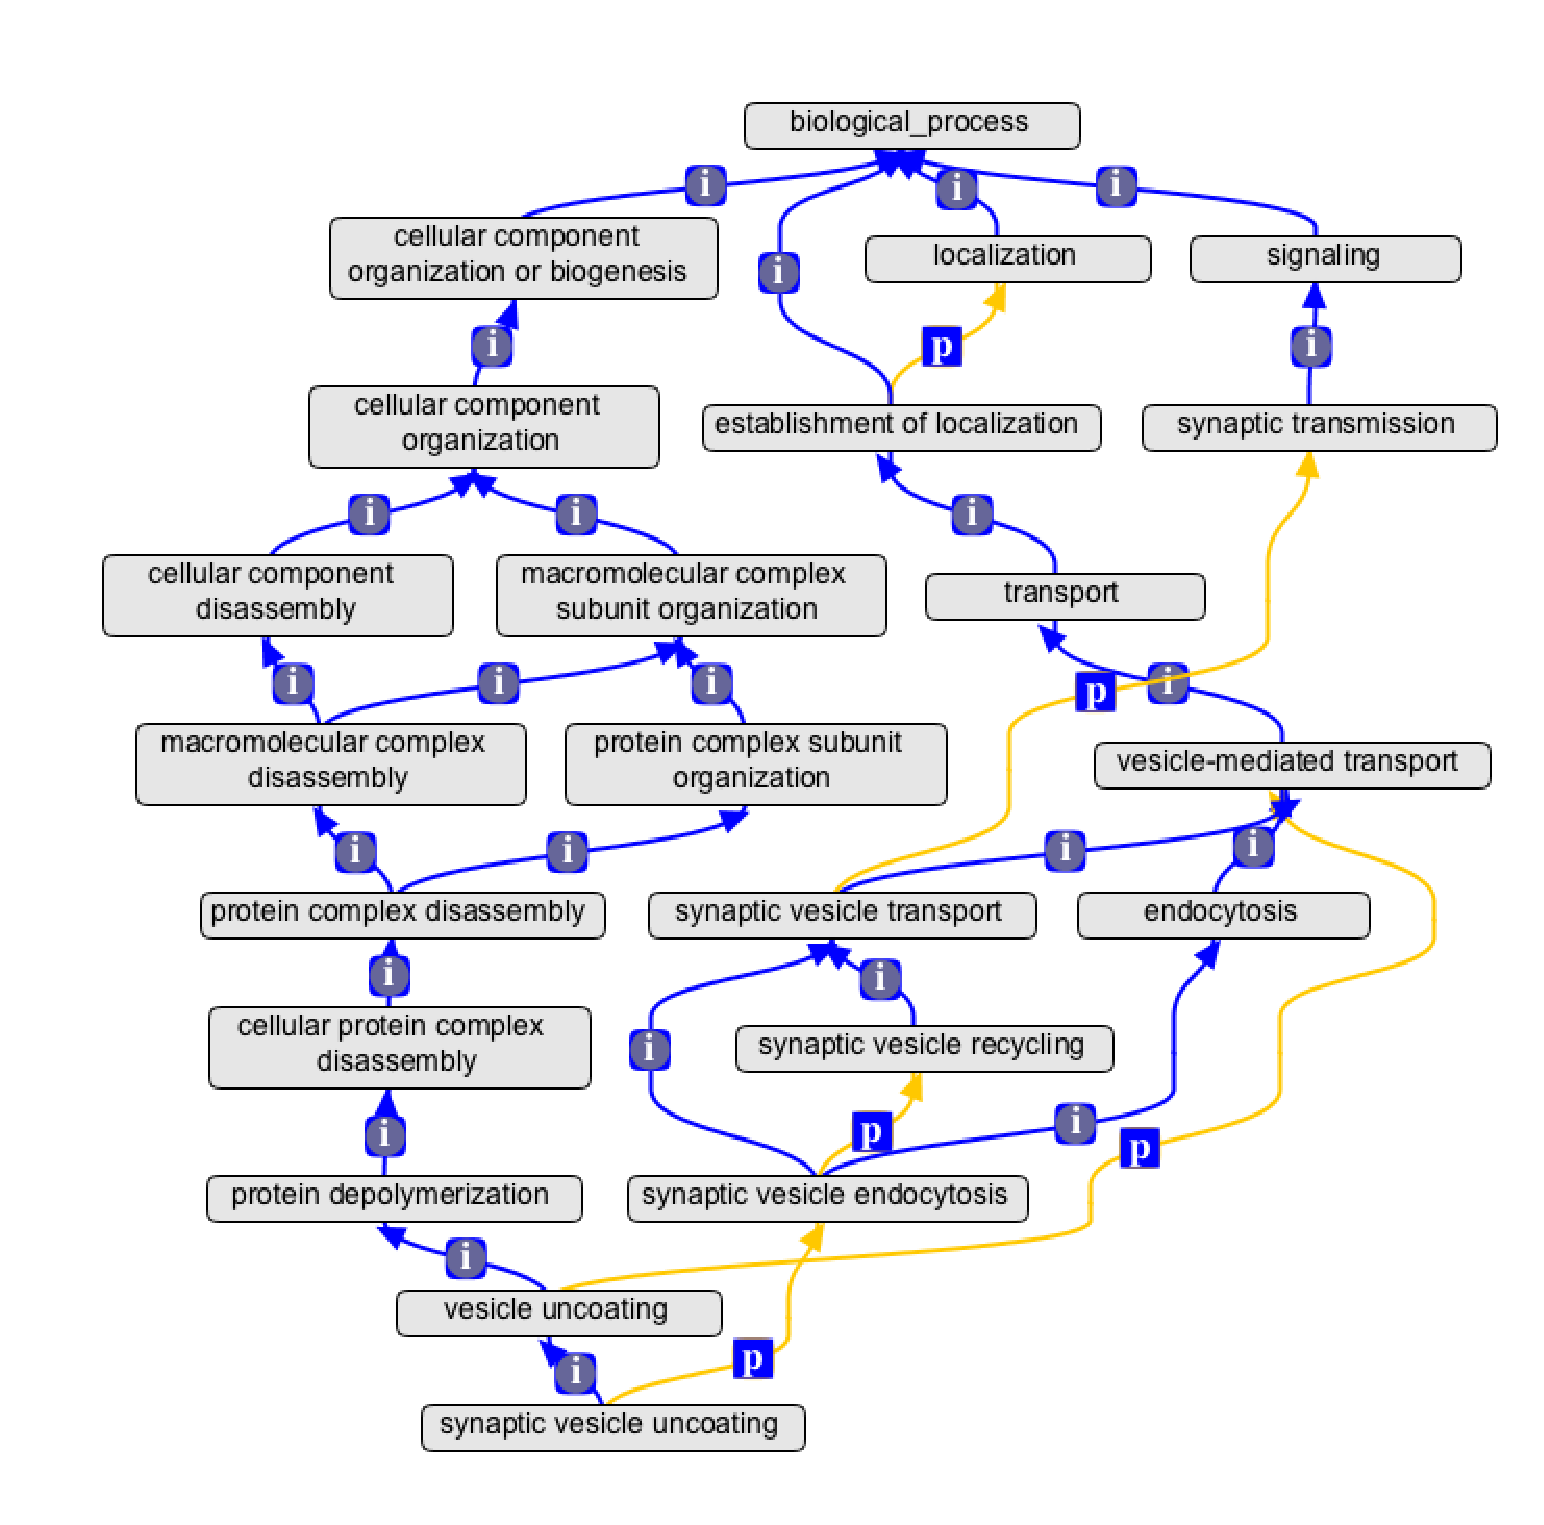
\includegraphics[height=4cm]{gv-plugin}
\caption{Figure 1: Protege GraphView plugin, ported from OBO-Edit}
\end{figure}
%----------------------------------------

% ----------------------------------------
\subsection{Web based templated term submission}
% ----------------------------------------

Biological data curators frequently need new classes for describing
the genes they are annotating. Often these classes fall into
particular compositional patterns with placement in the subsumption
hierarchy calculated automatically. In the past the sole method for
data curators to obtain new classes was through a sourceforge issue
tracking system, leading to bottlenecks.

To address this we created TermGenie\cite{Dietze2014}, a web-based
class submission system that allows curators to generate new classes
instantaneously, provided they pass a suite of logical, lexical and
structural checks. TermGenie submission can be according to either
pre-specified templates, or ``free-form'' submissions.

Currently we specify the templates procedurally as javascript code,
and we are currently exploring the use of Tawny-OWL\cite{Tawny} as the
templating engine.


% ----------------------------------------
\subsection{Smuggling OWL expressions into Databases}
% ----------------------------------------

In order to avoid overloading the ontology with two many named
classes, we have created an ``annotation extension'' system whereby
data curators can composed their own class expressions for describing
genes\cite{Huntley2014}. The expressivity of the system is
deliberately limited to refining a base class using one or more
existential restrictions.

This system has so far appeared to be a useful balance between
expressivity and simplicity. One problem is that data curation takes
place outside an OWL environment, so any logical errors (for example,
violation of a domain or range constraint) are not caught until the
curators submit their data to the central GO database, where we
perform reasoner-based validation.


% ----------------------------------------
\subsection{Ontology build pipeline}
% ----------------------------------------

As the GO evolved from being a single standalone artifact to modular
entity with a number of derived products we constructed an ontology
verification and publishing pipeline.

As is common in the bioinformatics world, we specify and execute our
pipeline using UNIX Makefiles, which allows the chaining together of
dependent tasks that consume and produce files.

We developed a command line utility that acts as a kind OWL Swiss-army
knife, with the original name of OWLTools\cite{OWLTools}. We developed
OWLTools according to the UNIX philosophy, with a view to integration
with Makefile-type pipelines. It is primarily a simple wrapper onto
the OWL API, and allows the execution of tasks such as checking if an
ontology is incoherent, generating ontology subsets and so on.

This pipeline is executed within a Continuous Integration
framework\cite{Mungall2012a}.

% ----------------------------------------
\subsection{Challenges of working with multiple ontologies}
% ----------------------------------------

We aim to follow the Rector Normalization patter, avoiding manual
assertion of poly-hierarchies, instead leveraging modular
hierarchies. Often these hierarchies fall in the domain of an ontology
external to GO, which presents a number of challenges. This was one of
the original motivations for the creation of the Open Biological
Ontologies (OBO) library, to lower the barrier for interoperation, by
ensuring all federated ontologies were open, orthogonal and responsive
to any requirements for improvement or change. Even with these
barriers lowered, challenges remain. Ontologies developed by different
groups often reflect different perspectives, design patterns and
hidden assumptions that can be hard to reconcile. The initial
axiomatization of one ontology using another often reveals multiple
unsatisfiable classes and invalid inferences. This can be
time-consuming to repair. The key here is early, prospective
integration, rather than after-the-fact.

There is also a deficit of tooling to support working in a
multi-ontology environment. Naive construction of import chains
results in highly inefficient transfer of large RDF/XML files over the
web. The resulting infrastructure is fragile, with multiple points of
failure. Versioning becomes of paramount importance, because simple
changes in an imported ontology can wreak havoc, causing mass
unsatisfiability, or loss of crucial inferences. Multiple partial
solutions exist, but none are perfect. BioPortal provides URLs for
individual versions of ontologies, but require an API key, which does
not work well with owl imports.

The parallels with software development are obvious. As ontologies
such as GO move from being monolithic to modular, we need the
equivalent of dependency management and build tools such as Maven, and
we welcome efforts such as the recent OntoMaven
project\cite{paschke2013ontomaven}.

Biological ontologies do not always modularize as cleanly as software
libraries. For example, there are multiple mutual dependencies between
the cell type ontology and GO (the former relies on the latter to
describe what cells have evolved to do, the latter relies on the
former to describe the development of these cells). This presents
additional challenges.

% Danger of circular dependencies.  Need for ontology equivalent of Maven...


% ========================================
\section{Future developments}
% ========================================

% ----------------------------------------
\subsection{Getting OWL into the mainstream}
% ----------------------------------------

We are highly dependent on OWL as part of the ontology development
cycle in GO. Axiomatization using equivalence and disjointedness
axioms are crucial for automating classification and quality
control. However, OWL axioms currently play less of a role once the ontology
is deployed and used. There are large numbers of highly sophisticated
analysis tools that incorporate the GO - most of these just treat the
ontology as a simple DAG (in fact a considerable number of tools drop
even this limited axiomatization, and just use the GO as a flat list
of terms). We believe there is a missed opportunity here. Some of this
may be in part due to the high barrier of entry for using OWL
(e.g. lack of native API in languages frequently used by
bioinformaticians, such as Python). This may also represent an
research opportunity for algorithms that combine the types of
statistical and probabilistic reasoning common in biology with
powerful deductive reasoning offered by description logics.

% ----------------------------------------
\subsection{Rise of the ABox}
% ----------------------------------------

Most of the detailed axiomatization in the GO represents the low
hanging fruit, such as equivalence axioms for compositional
concepts. Other aspects of biology are more resistant to
axiomatization - for example, multi-step pathways or complex cellular
processes such as apoptosis. The tree-model property of TBoxes makes
it impossible to faithfully encode multiply connected mechanistic
processes. The existence of high degrees of variability and exceptions
across different species presents challenges for a monotonic logical
encoding.

One approach we are exploring here is to utilize the ABox to represent
``prototypical'' biological processes. We have developed a web-based
graphical ABox editor called
Noctua\footnote{https://github.com/kltm/go-mme} for exploration of
this paradigm. Whilst the use of an ABox to represent knowledge
lessens the power of our model for deductive inferences, it represents
an opportunity for exploration of other models of inference that may
be more appropriate for biological systems.

% ========================================
\section{Conclusions}
% ========================================

The OWL language and tools have benefited the GO tremendously,
particularly the ontology development cycle and the validation of data
about genes. At this time, GO primarily uses a subset of OWL that is
supported by Elk, providing us the benefits of fast reasoning. In
general, like many biological ontologies, the GO is not in need of
esoteric extensions to OWL, but would benefit substantially from the
creation of new tools and the hardening of existing tools,
particularly related to release management.





% mention stress-testing with OWLAPI


% ========================================
\bibliography{go-owled-paper}
\bibliographystyle{plain}
% ========================================


\end{document}
